\tikzstyle{n}=[]%[xshift=.5cm, yshift=.5cm]
\tikzstyle{idx}=[font=\bfseries]
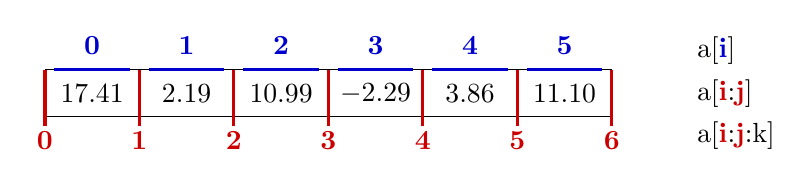
\begin{tikzpicture}[scale=.6, xscale=2]
  %\foreach\i in {0,1,2,3}{
  %  \draw[a] (.1, {0 + .5}) -- ++(4.2, 0);
  %  \draw[a] ({0 + .5}, .1) -- ++(0, 4.2);
  %}

  \draw (0, 0) grid (6, 1);
  \node[n] at (0.5, 0.5) {17.41};
  \node[n] at (1.5, 0.5) { 2.19};
  \node[n] at (2.5, 0.5) {10.99};
  \node[n] at (3.5, 0.5) {$-$2.29};
  \node[n] at (4.5, 0.5) { 3.86};
  \node[n] at (5.5, 0.5) {11.10};

  \foreach\i in {0,...,5} {
    \draw[very thick, blue!80!black] ({\i + .1}, 1) -- ({\i + .9}, 1);
    \node[idx, blue!80!black] at ({\i + .5}, 1.5) {\i};
  }
  \foreach\i in {0,...,6} {
    \draw[very thick, red!80!black] (\i, -0.2) -- (\i, 1);
    \node[idx, red!80!black] at (\i, -.5) {\i};
  }

  \node[anchor=west] at (6.8,  1.4) { a[\textcolor{blue!80!black}{\textbf{i}}] };
  \node[anchor=west] at (6.8,  0.5) { a[\textcolor{red!80!black}{\textbf{i}}:\textcolor{red!80!black}{\textbf{j}}] };
  \node[anchor=west] at (6.8, -0.4) { a[\textcolor{red!80!black}{\textbf{i}}:\textcolor{red!80!black}{\textbf{j}}:k] };

\end{tikzpicture}

